% Chapter 3 - Results 

\chapter{Results} % Main chapter title

\label{chap:results} % For referencing the chapter elsewhere, use \ref{Chapter1} 

\lhead{Chapter 3. \emph{Comparison of methods}} % This is for the header on each page - perhaps a shortened title

%----------------------------------------------------------------------------------------
\section{The main differences}
Using least squares will always give you a SPD system of equations which can be advantageous. However for second order equations this system is three times as big as if we were to solve it using more standard methods. Comparing the correctness of the solution as done in figure ~\ref{fig:convergence} shows that the convergence rate is the same as for standard methods, but the the value of the residual is slightly higher for the least squares method. This can be explained by the functional that is minimized. Notice that in the least squares methods you minimize the square of the residual. since the correctness of both methods are restricted by the smoothness of the solution and the number of discrete points LS-methods will minimize the residual squared down to a given precision and hence the residual itself to a slightly higher value. 
%
\begin{figure}[hl]
	\centering
	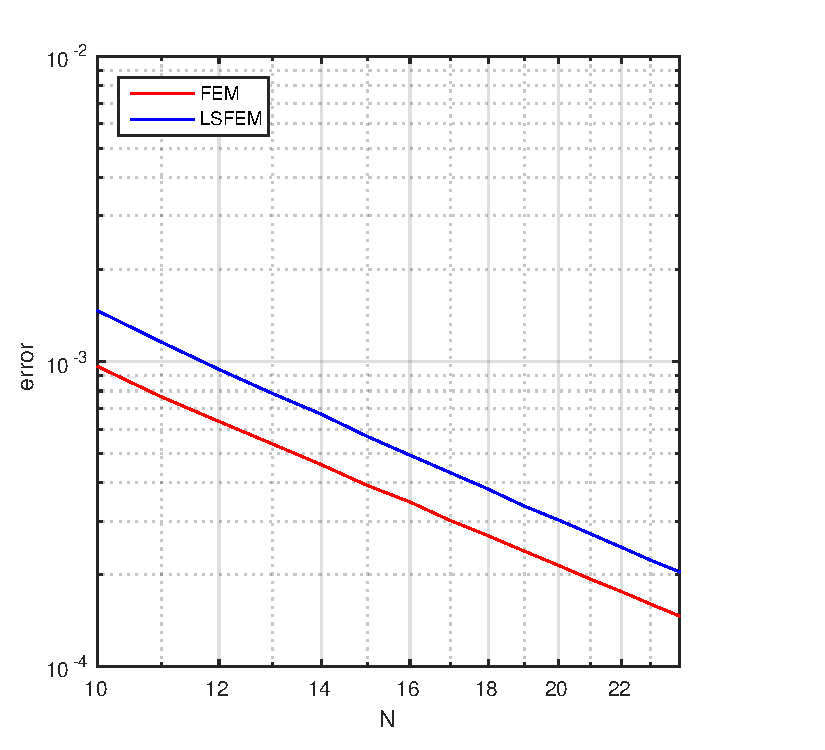
\includegraphics{Figures/errorFEM-LSFEM.pdf}
	\caption{convergence of LSFEM and FEM}
	\label{fig:convergenceFEM}
\end{figure}
%
The condition number is also worth comparing \ldots
%
\begin{figure}[hl]
	\centering
	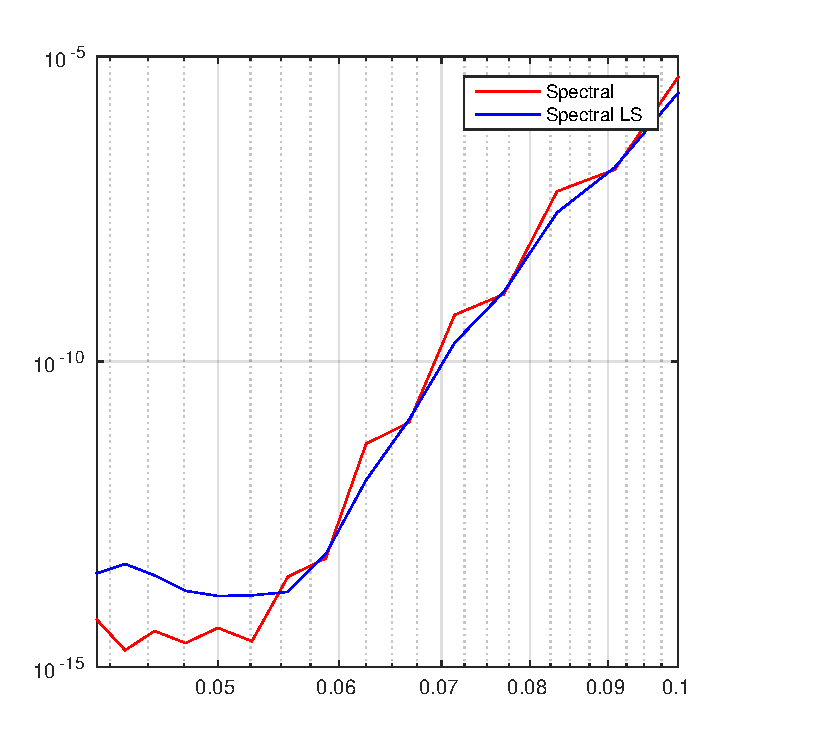
\includegraphics{Figures/errorSpec-SpecLS.pdf}
	\caption{convergence of Spectral and LS-Spectral method}
	\label{fig:convergenceSpec}
\end{figure}
%
%
\begin{figure}[hl]
	\centering
  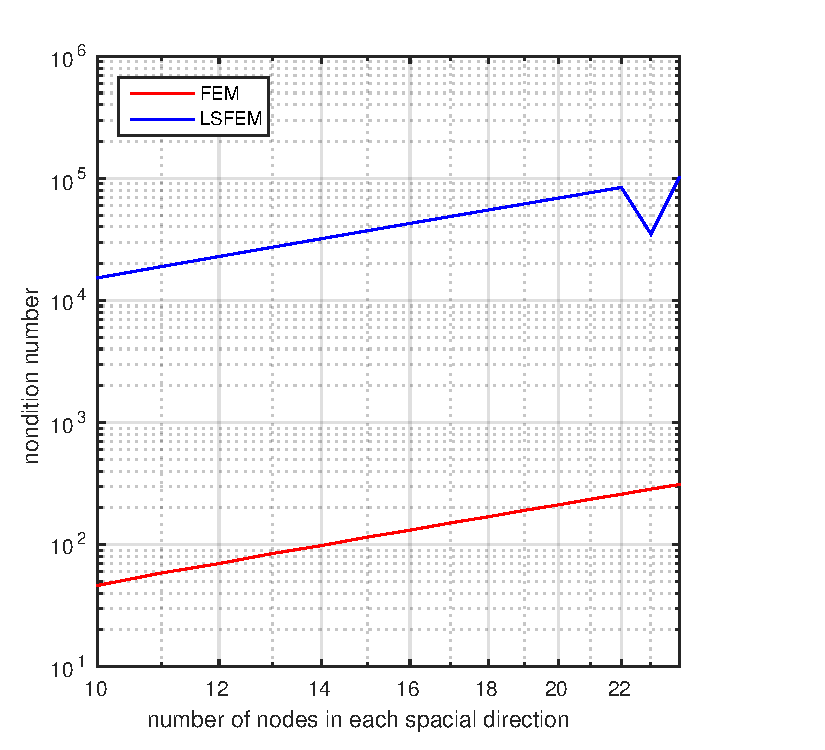
\includegraphics{Figures/condFEM-LSFEM.pdf}
	\caption{condition number of LSFEM and FEM}
	\label{fig:conditionFEM}
\end{figure}
%
%
\begin{figure}[hl]
	\centering
	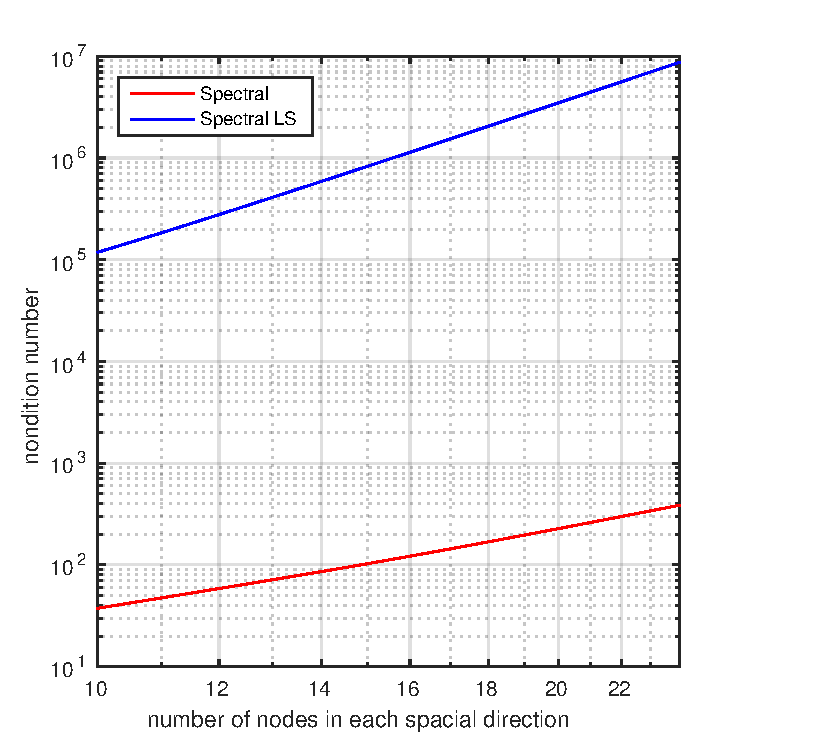
\includegraphics{Figures/condSpec-SpecLS.pdf}
	\caption{condition number of Spectral and LS-Spectral method}
	\label{fig:conditionSpec}
\end{figure}
%

